%!TEX encoding = UTF-8 Unicode
\documentclass{lecturenotes}

\setbeamertemplate{footline}[frame number]
\title[Scala as a beginner language]{Scala as a beginner language}
\subtitle{-- Experiences and plans at LTH}
\author{Björn Regnell}
\institute{Dept. of Computer Science, LTH \\ Lund University, Sweden}
\date{2016 April 20}

\begin{document}

\frame{\titlepage}
\frame{\Emph{Agenda}\tableofcontents}

%%% EXPERIENCES

\section[Experiences with Scala at LTH]{Experiences with Scala as a beginner language at LTH}

\subsection[Scala at LTH Science Center Vattenhallen]{Primary school activities at LTH Vattenhallen}

\begin{Slide}{Primary school activities at LTH Science Center Vattenhallen}
\begin{multicols}{2}

\footnotesize
\begin{itemize}
\item \Alert{Thousands of school kids} visiting Vattenhallen have done \Emph{programming experiements} using LTH's free teaching material in Scala and Kojo:
\href{http://www.lth.se/programmera/uppdrag}{www.lth.se/programmera/uppdrag} \\ \Alert{Try it yourself!}

\item \Alert{Hundreds of teachers} have taken LTH's \Emph{programming courses for teachers} 

\item LTH is supporting \Emph{Skolverket} in dev of coming curricula. \\\Alert{AT LAST:}\\ \Emph{Programming in school!!!}




\end{itemize}
\columnbreak
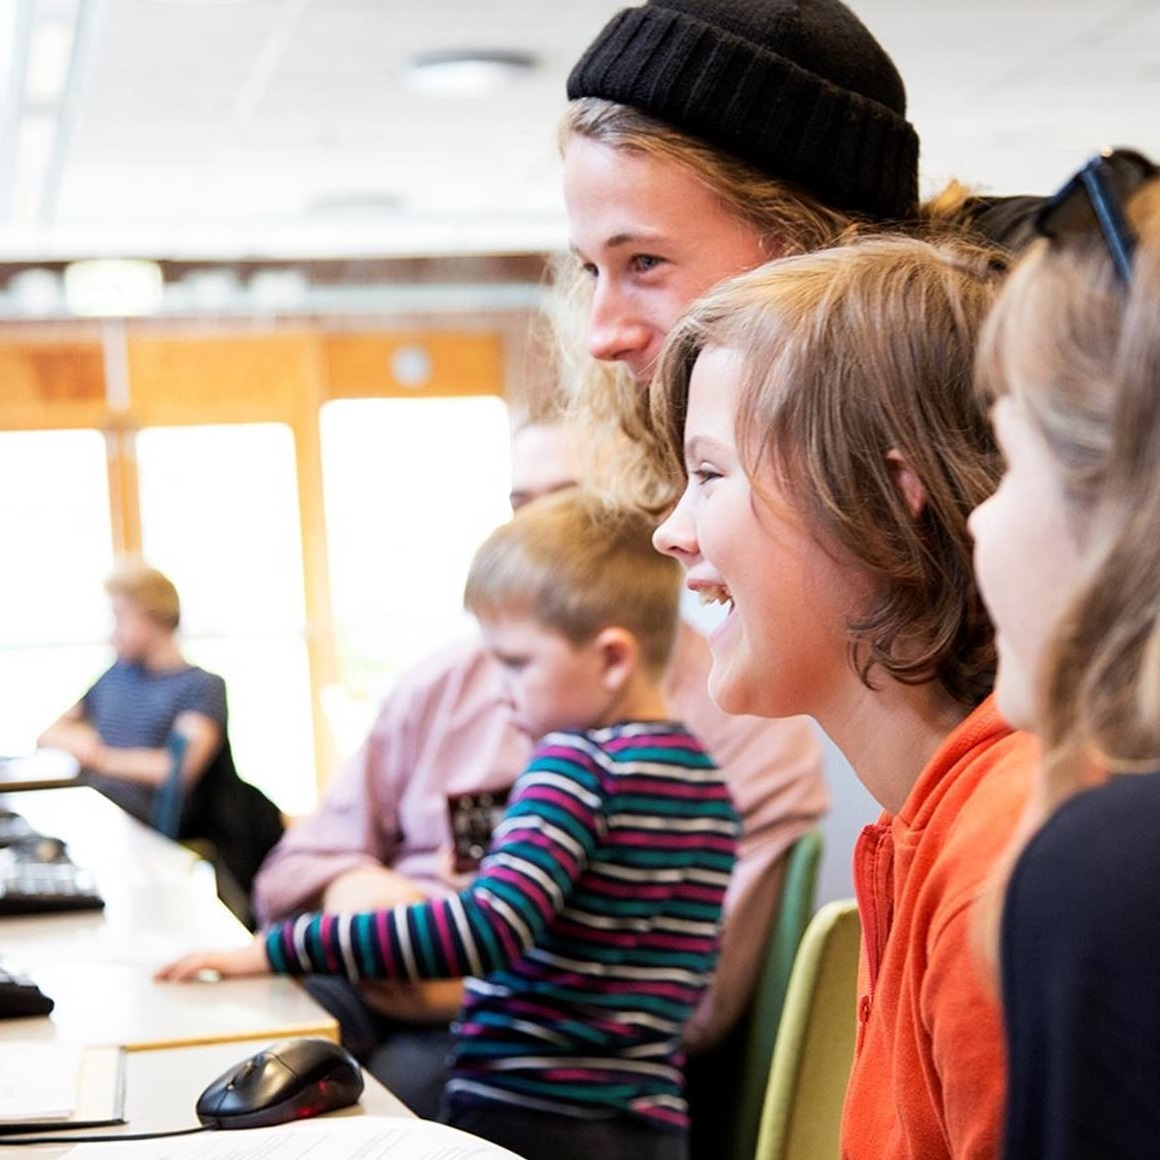
\includegraphics[width=0.6\textwidth]{../../img/kids}
\end{multicols}

\end{Slide}

\subsection[Turtle graphics in Scala with Kojo]{Turtle graphics in Scala with Kojo in Swedish}

\begin{Slide}{Programing for Kids in school}
\begin{multicols}{3}
\begin{itemize}
\item \Alert{S}equence
\item \Alert{A}lternative
\item \Alert{R}epetition
\item \Alert{A}bstraction
\end{itemize}
\columnbreak
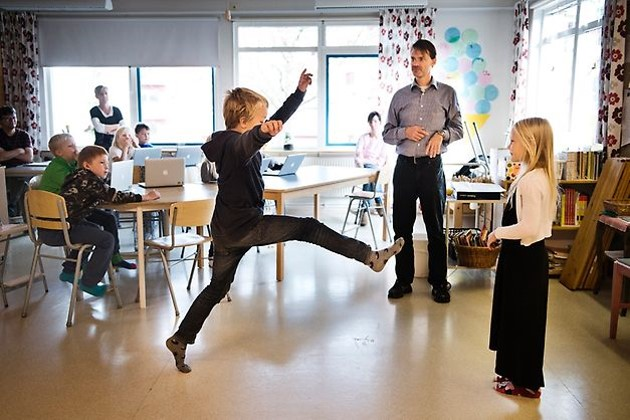
\includegraphics[width=0.7\textwidth]{../../img/unplugged}
\end{multicols}
\end{Slide}


\begin{Slide}{Scala for Kids: Turtle graphics in Kojo}
\begin{multicols}{2}
\begin{itemize}
\item \Alert{S}equence
\item \Alert{A}lternative
\item \Alert{R}epetition
\item \Alert{A}bstraction
\end{itemize}
\columnbreak
{
\includegraphics[width=0.5\textwidth]{../../img/kojo/stairs}}
\end{multicols}
\end{Slide}


\begin{Slide}{Experiences with Scala for kids}
\begin{itemize}
\item Good, evolving, easy-to-use IDE available: \\ \Emph{Kojo} -- try it yourself: 
\href{http://www.kogics.net/kojo}{www.kogics.net/kojo-download}
\item Fulfills three important criteria: 
\begin{itemize}
\item \Emph{Free} and open source; schools don't have to pay
\item Available \Emph{in Swedish}; identifyers with öåä
\item Programming ''\Emph{for real}''; the sky is the limit...
\end{itemize}
\item Avoids beginner-unfriendly boilerplate, e.g.: \\ \texttt{public static void main(String[] args)}
\item Flexible syntax and powerful language constructs that enbale creation of \Emph{simple} control structures:
\begin{Code}
upprepa(10){ fram; höger }
\end{Code}
\item Concise syntax and low ''cost'' of \Emph{abstraction}
\begin{Code}
def kvadrat = upprepa(10){ fram; höger }
\end{Code}
\end{itemize}
\end{Slide}

%%% PLANS

\section[Plans for Scala at LTH]{Future plans for Scala as a beginner language at LTH}

\begin{Slide}{On-going curicula development of CS courses}
Four new courses for the CSE program (Datateknik):
\begin{itemize}
\item Introduction to computer programming (Scala+Java)
\item Evaluation of software systems (R)
\item Discrete structures in computer science (Clojure)
\item Functional programming (Lang. TBD)
\end{itemize}
\vspace{1em} More information:
\url{http://cs.lth.se/education/}
\end{Slide}

\subsection[Potential pedagogical benefits and risks]{Potential pedagogical benefits and risks}

\begin{Slide}{Why Scala?}
Potential \Emph{benefits}:
\begin{itemize}\fontsize{9}{10}\selectfont
\item Regular semantics, e.g. no dicotomy btw primitive types \& objects
\item Concise, expressive syntax: don't get drowned in a ''letter soup''
\item Interactive learning through experiments in the Scala REPL
\item Multi-paradigm, pragmatic: imperative, object-oriented, functional
\item Rich semantics: can demonstrate many modern, advanced cs concepts
\item New, modern, evolving language exciting for new students
\item Also non-beginners get a challange 
\item Free, open source language and tools
\end{itemize}
Potential \Alert{risks}:
\begin{itemize}\fontsize{9}{10}\selectfont
\item Tools not becoming mature fast enough?  
\item Lack of beginner-oriented teaching material?
\item Future industrial relevance? 
\item Critical mass of community?
\end{itemize}
\end{Slide}


\begin{Slide}{Course intro survey 2015, CSE (Datateknik)\\EDA016 Programming, first course (Java)}
\begin{multicols}{2}
Have programmed before? \vspace{1em}

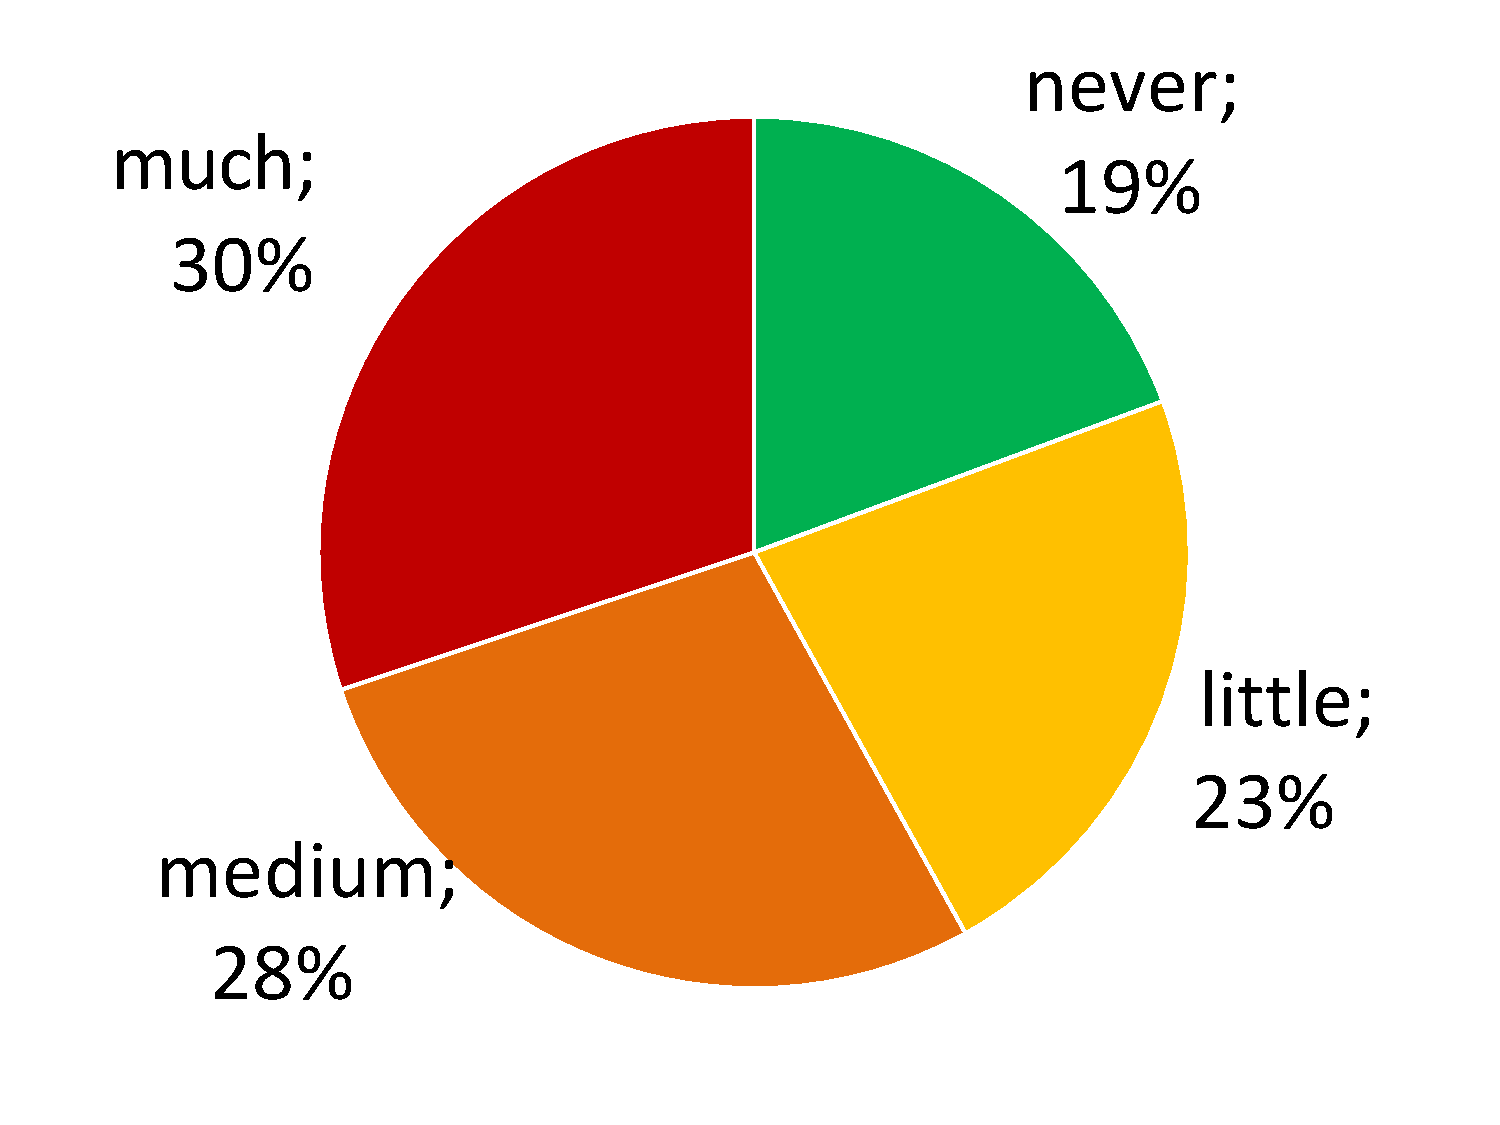
\includegraphics[width=0.55\textwidth]{img/survey-2015}
\columnbreak

\raggedleft What language?  \vspace{1em}

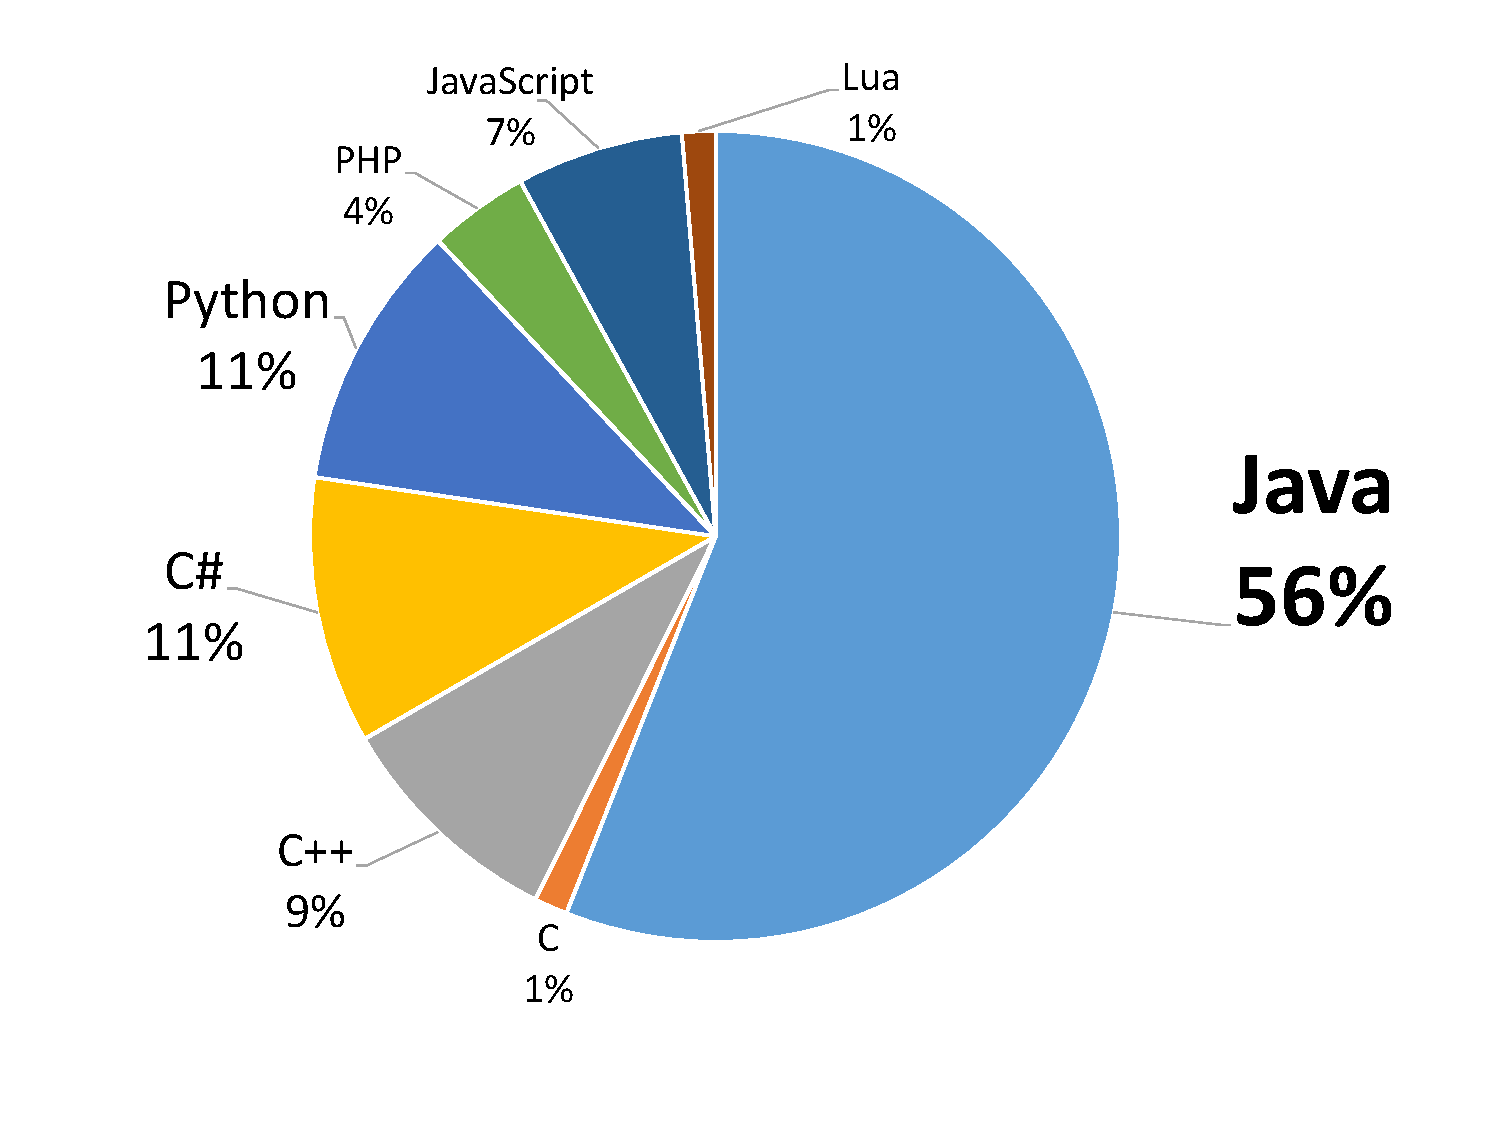
\includegraphics[width=0.55\textwidth]{img/lang-2015}
\end{multicols}
\end{Slide}


\begin{Slide}{Course results 2015, CSE (Datateknik)\\EDA016 Programming, first course (Java)}
\begin{multicols}{2}

\Emph{Grades D-program 2015}  \vspace{1em}

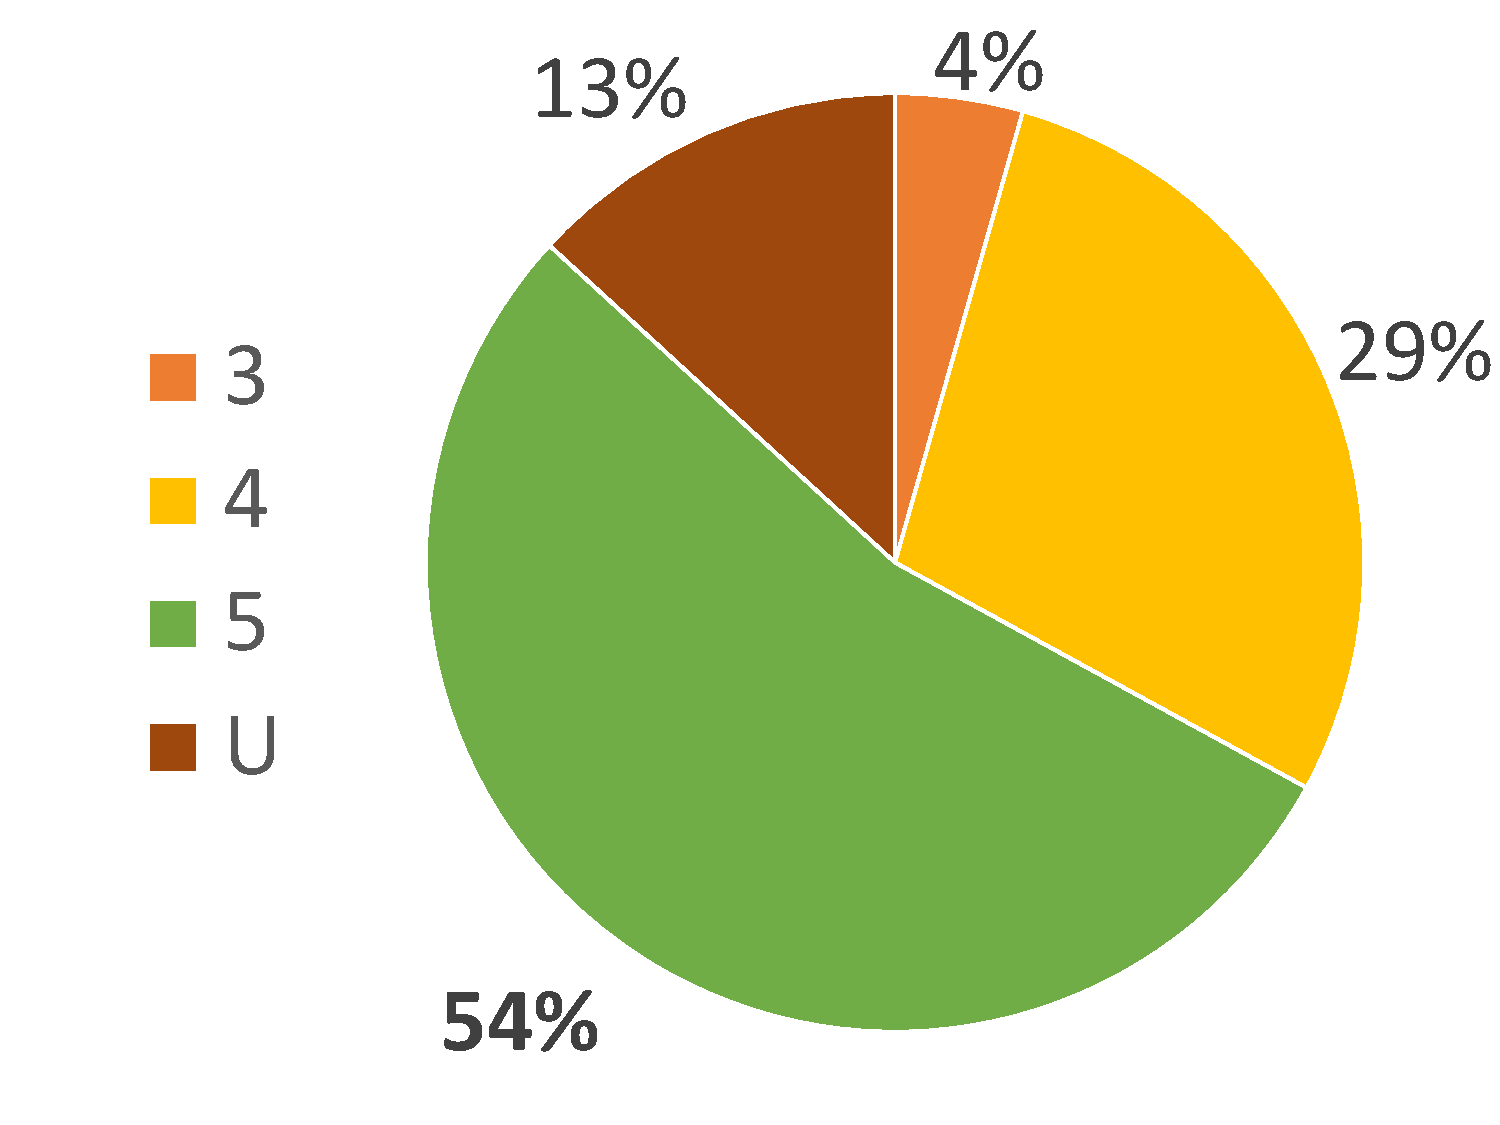
\includegraphics[width=0.55\textwidth]{img/grades-2015}

\columnbreak

\raggedleft \Emph{Goal of 2016} \\
To \Alert{increase} the \\ \Alert{challenge level} \& \\  \Alert{learning outcome} \\ significantly.
\end{multicols}
\end{Slide}

\subsection[New course: EDAA45 ''Introduction to programming'']{New course: EDAA45 ''Introduction to programming''}


\begin{Slide}{New course: EDAA45 Introduction to programming \\ using Scala and Java}
\noindent\resizebox{0.8\columnwidth}{!}{
%!TEX encoding = UTF-8 Unicode
\begin{tabular}{l|l|l|l}
\textit{W} & \textit{Modul} & \textit{Övn} & \textit{Lab} \\ \hline \hline
W01 & Introduktion            & expressions & kojo            \\
W02 & Kodstrukturer           & programs    & --              \\
W03 & Funktioner, Objekt      & functions   & simplewindow    \\
W04 & Datastrukturer          & data        & textfiles       \\
W05 & Sekvensalgoritmer       & sequences   & cardgame        \\
W06 & Klasser, Likhet         & classes     & shapes          \\
W07 & Arv, Gränssnitt         & traits      & turtlerace-team \\
KS  & KONTROLLSKRIVN.         & --          & --              \\
W08 & Mönster, Undantag       & matching    & chords-team     \\
W09 & Matriser, Typparametrar & matrices    & maze            \\
W10 & Sökning, Sortering      & sorting     & surveydata-team \\
W11 & Scala och Java          & scalajava   & scalajava-team  \\
W12 & Trådar, Web, Android    & threads     & life            \\
W13 & Design                  & Uppsamling  & Inl.Uppg.       \\
W14 & Tentaträning            & Extenta     & --              \\
T   & TENTAMEN                & --          & --              \\
\end{tabular}

}
\end{Slide}


\begin{Slide}{Student participation in teaching development through open sourcing of teaching material for Scala}

{\large\textbf{\url{https://github.com/lunduniversity/introprog}}}

\begin{multicols}{3}\footnotesize
Anders Buhl, \\Anna Palmqvist Sjövall, \\Anton Andersson, \\Casper Schreiter, \\Cecilia Lindskog, \\Christine Boghammar, \\Emil Wihlander, \\Emma Asklund, \\Erik Bjäreholt, \\Erik Grampp, \\Erik Söderbarg, \\Filip Stjernström, \\Fredrik Danebjer, \\Gustav Cedersjö, \\Henrik Olsson, \\Jacob Bohlin, \\Jakob Hök, \\Johan Ravnborg, \\Jonas Danebjer, \\Maj Stenmark, \\Maximilian Rundgren, \\Måns Magnusson, \\Oscar Sigurdsson, \\Oskar Berg, \\Oskar Widmark, \\Povel Larsson, \\Sebastian Hegardt, \\Stefan Jonsson, \\Tom Postema, \\Valthor Halldorsson, \\Viktor Claesson
\end{multicols}

\Emph{Contributions are welcome!} {\footnotesize\url{mailto:bjorn.regnell@cs.lth.se}}
\end{Slide}

\section*{Scala crash course for you!}
\subsection*{Evening event by code@lth}

\begin{Slide}{Thank You!}
\Large \Emph{Welcome} to gasquesalen at 18:00 tonight for a Scala crash course with \Emph{code@lth} \\ \vspace{1em} \Alert{Free pizza} if you pre-register here:\\ \vspace{0.5em}  \url{http://goo.gl/forms/F2iME0j6Go}
\end{Slide}

\end{document}
